
% \begin{abstract}
% Implementing advanced vision models on edge devices is becoming progressively necessary for crucial applications, while it represents considerable obstacles due to severe computational restrictions, constrained battery longevity, and unstable network settings. Conventional static partitioning and independent model selection systems usually collapse under unanticipated resource surges and rapidly changing visual environments, resulting in substantial system faults and queue congestion. To resolve this lack of adaptability, we present an innovative multi-objective reinforcement learning framework. that establishes a cohesive Markov decision process for combined dynamic model adaptation and DAG-aware layer partitioning, leveraging both real-time hardware telemetry and lightweight image complexity metrics. [Result]. By tightly coupling visual characteristics and system telemetry with a farsighted RL policy, our approach provides a robust, fault-tolerant foundation that seamlessly optimizes the essential triadic trade-off concerning inference precision, end-to-end latency, and the power consumption of devices in unpredictable edge scenarios.

% \hl{(Note: Abstract length should be 150-170 words)}
% \end{abstract}

% \begin{IEEEkeywords}
% Edge computing, reinforcement learning, DNN partitioning, mobile vision, directed acyclic graph (DAG)
% \end{IEEEkeywords}


\section{Introduction}

Retrieval-Augmented Generation (RAG) has emerged as a highly successful paradigm to alleviate factual hallucinations and ground Large Language Models (LLMs) in external document collections. However, traditional vector RAG typically operates on chunk-based linear document slices that lack structural semantic connections and struggle with complex multi-hop queries. To address this, GraphRAG structures unstructured text as entity-relation graphs and hierarchical community summaries to support comprehensive global reasoning \cite{edge2024local}. Concurrently, Reinforcement Learning (RL) has shown great potential in training language models to make sequential decisions and navigate complex retrieval spaces . By formulating retrieval and reasoning as Markov Decision Processes and optimizing policies using environmental task-level rewards, RL provides a dynamic optimization mechanism to adapt static graph structures for downstream utility \cite{tsang2026autographr1}.

A rich line of research has explored learning-based graph reduction, sparsification, and context compression to handle the scale of complex graphs . In graph reduction, frameworks such as SparRL and Cutter \cite{chai2025cutter} leverage RL to prune non-essential edges and nodes to preserve graph robustness and topological properties \cite{hashemi2024comprehensive} . For context compression, methods like CORE \cite{cui2025core} and DynaRAG \cite{zhang2026dynarag} utilize RL to adaptively compress textual contexts based on downstream task performance . More recently, RL has been integrated directly into knowledge graph construction (AutoGraph-R1 \cite{tsang2026autographr1}) and agentic multi-turn GraphRAG reasoning (Graph-R1 \cite{luo2026graphr1} and GraphRAG-R1 \cite{yu2026graphragr1}) to optimize generation quality, retrieval relevance, and reasoning path correctness.

Despite these substantial advances, existing frameworks suffer from critical bottlenecks. First, traditional graph sparsification and reduction methods remain decoupled from downstream generator requirements, optimizing instead for task-agnostic, intrinsic topological metrics like degree or density. Second, current GraphRAG pipelines incur significant computational and token overhead from encoding entire retrieved subgraphs or dense community summaries at inference time. Third, existing schemas rely on rigid, predefined heuristics or hop counts, failing to adaptively compress graph contexts based on the specific semantic complexity of each query.

To resolve these limitations, we introduce an end-to-end framework for Adaptive Graph Compression using Reinforcement Learning for Efficient GraphRAG. Rather than task-agnostic preprocessing, our framework directly aligns graph reduction with downstream question-answering utility using direct generator feedback. Specifically, we address the core challenges of structural redundancy, massive token overhead, and rigid retrieval schemes. Our key contributions are summarized as follows:

\begin{itemize}
    \item \textbf{Query-Adaptive Graph Compression Policy:} We introduce a reinforcement learning-based graph compression policy that dynamically prunes retrieved subgraphs on the fly, tailoring the residual graph structure to meet the specific semantic demands of each user query.
    \item \textbf{Process-Constrained Joint Reward Mechanism:} We design a joint reward function that integrates downstream question-answering performance with token-level efficiency constraints. This process-constrained mechanism dynamically balances reasoning depth and computational overhead, preventing both shallow retrieval and over-thinking.
    \item \textbf{High-Fidelity Context Compression:} We evaluate our framework on multi-hop benchmarks against non-adaptive pruning baselines to assess whether substantial context compression ratios (significantly reducing context lengths at inference time) can be achieved while maintaining or improving downstream reasoning accuracy; we report this comparison directly, including cases where the learned policy has not yet surpassed simpler baselines at current training scale, as an honest account of the trade-off rather than a claim assumed in advance.
\end{itemize}

The remainder of this paper is organized as follows. Previous work on Graph Retrieval-Augmented Generation (GraphRAG), graph reduction and sparsification, and reinforcement learning for context optimization is reviewed in Section \ref{sec:RW}. Section \ref{sec:PS} details the proposed system model, including the Markov Decision Process (MDP) formulation for query-adaptive graph compression, the formal definitions of the state and action spaces, and the design of the process-constrained reinforcement learning agent. Section \ref{sec:ERD} presents the experimental setup and analyzes the system's performance specifically focusing on context compression ratios and downstream question-answering accuracy against state-of-the-art baselines on complex multi-hop benchmarks. The limitations of the proposed framework and future research directions are discussed in Section \ref{SEC: limF}, leading to Section \ref{sec:con} which concludes the paper.



\section{Related Work}
\label{sec:RW}

The paradigm of Retrieval-Augmented Generation (RAG) has substantially advanced the applicability of Large Language Models (LLMs) by prepending relevant external documents to the user query, successfully reducing factual hallucinations and grounding model outputs \cite{edge2024local, cui2025core}. However, traditional vector-based RAG approaches are typically restricted to flat, chunk-based document segments that fail to capture high-order semantic relationships among entities, making them ill-suited for complex multi-hop queries or global corpus summarization \cite{luo2026graphr1, edge2024local}. To address these limitations, \citet{edge2024local} pioneered the GraphRAG framework, which constructs structured entity-relationship graphs from raw text and partitions them hierarchically using Leiden community detection. Nonetheless, a major limitation of the approach by \citet{edge2024local} is that the graph construction and community-summarization processes are entirely heuristic and lack a learned compression policy, frequently resulting in severe token bloat and massive computational overhead at inference time. To balance hierarchical retrieval with adaptive semantic integration, \citet{li2026deepgraphrag} proposed Deep GraphRAG to maintain local precision and global context. However, the model designed by \citet{li2026deepgraphrag} applies conciseness or semantic weight rewards primarily to textual summaries rather than performing any adaptive structural compression on the underlying graph topology. Towards dynamic and agentic retrieval pipelines, \citet{luo2026graphr1} proposed Graph-R1, which models the retrieval process as an agentic, multi-turn loop over a knowledge hypergraph. Concurrently, \citet{yu2026graphragr1} developed GraphRAG-R1, which leverages process-constrained reinforcement learning (RL) with progressive retrieval attenuation to guide tool invocation. Despite their reasoning gains, both \citet{luo2026graphr1} and \citet{yu2026graphragr1} focus exclusively on optimizing the step-by-step retrieval navigation policy, leaving the retrieved graph or hypergraph size fixed and uncompressed, which still subjects the downstream generator to significant token overhead.

To handle the scaling bottlenecks associated with large-scale graph databases, graph reduction has emerged as a key preprocessing step to compress networks while preserving vital properties, as detailed in the comprehensive survey by \citet{hashemi2024comprehensive}. However, as a literature survey, the work of \citet{hashemi2024comprehensive} does not propose an empirical methodology of its own nor does it address task-specific downstream generation requirements. In the domain of learning-based sparsification, \citet{wickman2022sparrl} proposed SparRL, which trains deep reinforcement learning agents to prune non-essential edges. Nevertheless, the framework by \citet{wickman2022sparrl} relies on a purely structural reward (e.g., preserving PageRank or community structures) and is not evaluated on any downstream semantic question-answering task, which makes it task-agnostic. Expanding on structural robustness under targeted node-deletion attacks, \citet{chai2025cutter} developed Cutter, which utilizes a dual-agent RL architecture consisting of a node detector and an edge compressor. However, similar to other sparsification baselines, \citet{chai2025cutter} optimize their agents solely for topological connectivity metrics in a structure-only setting, ignoring the semantic and task-specific demands of downstream LLM generators.

Parallel to structural reduction, several works have focused on task-aligned context compression and index optimization. In document context compression, \citet{cui2025core} proposed CORE, an end-to-end framework that leverages Group Relative Policy Optimization (GRPO) to condense retrieved text down to 3\% of its original length based on downstream task-level feedback. Similarly, \citet{zhang2026dynarag} developed DynaRAG, employing reinforcement learning to adaptively select context compression ratios according to dynamic query demands. Although highly effective at reducing inference cost, both \citet{cui2025core} and \citet{zhang2026dynarag} operate strictly on flat, unstructured text chunks and are incapable of exploiting or preserving graph-structured topologies. To bridge the gap between graph index building and downstream performance, \citet{tsang2026autographr1} presented AutoGraph-R1, which formulates knowledge graph construction as a policy learning problem optimized via GRPO. However, \citet{tsang2026autographr1} optimize the triple generation process exclusively at construction time; their method lacks a post hoc mechanism to compress the retrieved subgraph size dynamically during query execution. Our work bridges these disparate lines of research by learning a query-adaptive graph compression policy that dynamically prunes retrieved subgraphs on the fly, optimizing downstream generation accuracy and inference token efficiency in unison.

\begin{table*}[!t]
\centering
\caption{Summary of related studies on reinforcement learning for graph compression and GraphRAG optimization}
\label{tab:related_work}
\resizebox{\textwidth}{!}{%
\begin{tabular}{c c p{3.2cm} p{4.5cm} p{3.6cm} p{3.8cm}}
\toprule
\textbf{Ref.} & \textbf{Year} & \textbf{Method / Algorithm} & \textbf{Dataset} & \textbf{Results} & \textbf{Limitations} \\
\midrule

{\cite{wickman2022sparrl}} &
2022 &
MDP-based edge sparsification with user-specified reward. &
Generic benchmark graphs (structural evaluation, no QA corpus). &
Consistent gains over sampling-based sparsification baselines across structural objectives. &
Purely structural reward; not evaluated on any retrieval-and-generation task. \\

{\cite{edge2024local}} &
2024 &
Heuristic LLM-based entity-relation extraction with Leiden community partitioning. &
Podcast transcripts and MultiHop-RAG corpora. &
Enables query-focused summarization across large corpora via community summaries. &
Construction and reduction are entirely heuristic; no learned compression policy. \\

{\cite{cui2025core}} &
2025 &
End-to-end GRPO-trained context compressor rewarded by downstream accuracy. &
Four open-domain QA datasets. &
3\% compression ratio with a 3.3-point average EM gain over uncompressed context. &
Operates on flat, unstructured text; no graph topology exploited. \\

{\cite{chai2025cutter}} &
2025 &
Dual-agent RL (Vital Detection + Redundancy Detection) with shared GCN encoder. &
Generic benchmark graphs (topological robustness evaluation). &
Preserves topological robustness profile of graphs under aggressive compression. &
Structural robustness objective only; not tailored to retrieval or GraphRAG. \\

{\cite{tsang2026autographr1}} &
2026 &
GRPO-fine-tuned LLM triple extractor rewarded by downstream retrieval utility. &
HotpotQA, MuSiQue, 2WikiMultihopQA, NQ, PopQA. &
Up to +4.39 average F1 gain over zero-shot construction across retrieval paradigms. &
Optimizes graph content at construction time; does not reduce graph size post hoc. \\

{\cite{yu2026graphragr1}} &
2026 &
Modified GRPO with Progressive Retrieval Attenuation and Cost-Aware F1 rewards. &
HotpotQA, 2Wiki, MuSiQue, PopQA. &
Up to 38.08--83.81\% F1 improvement over strongest baselines across datasets. &
Optimizes retrieval-invocation policy only; graph size remains fixed. \\

{\cite{luo2026graphr1}} &
2026 &
Multi-turn agentic RL (GRPO) over a lightweight knowledge hypergraph. &
2WikiMultiHopQA, HotpotQA, Musique, NQ, PopQA, TriviaQA. &
Outperforms chunk- and graph-based RL baselines in F1 across all six benchmarks. &
Retrieval-policy optimization only; hypergraph construction remains lightweight/heuristic. \\

{\cite{zhang2026dynarag}} &
2026 &
MDP-based per-chunk compression ratio selection via Thompson Sampling. &
Multi-retriever QA benchmarks (Contriever, BGE-M3, BM25, Hybrid). &
18.53\% knowledge-base storage reduction with an 8.31\% DCG@1 improvement. &
Operates on flat text chunks; no structural graph-reduction operators. \\

{\cite{li2026deepgraphrag}} &
2026 &
Dynamically-Weighted GRPO (DW-GRPO) for adaptive multi-objective reward balancing. &
Natural Questions, HotpotQA. &
Compact 1.5B model approaches large-model performance in knowledge integration. &
Conciseness reward applied to summary text, not to graph structure. \\

\bottomrule
\end{tabular}}
\end{table*}



\section{Methodology}\label{sec:PS}

The proposed framework addresses inefficient task-agnostic graph retrieval in GraphRAG pipelines by introducing a learned, query-adaptive compression stage between retrieval and generation. The overall pipeline, illustrated in Fig.~\ref{fig:workflow}, consists of six stages: (1) dataset and knowledge graph construction, (2) query representation and GraphRAG retrieval, (3) answer generation from the retrieved graph, (4) GRPO-based query-adaptive graph compression, (5) compressed answer generation and reward, and (6) performance and evaluation.

\begin{figure*}[!t]
    \centering
    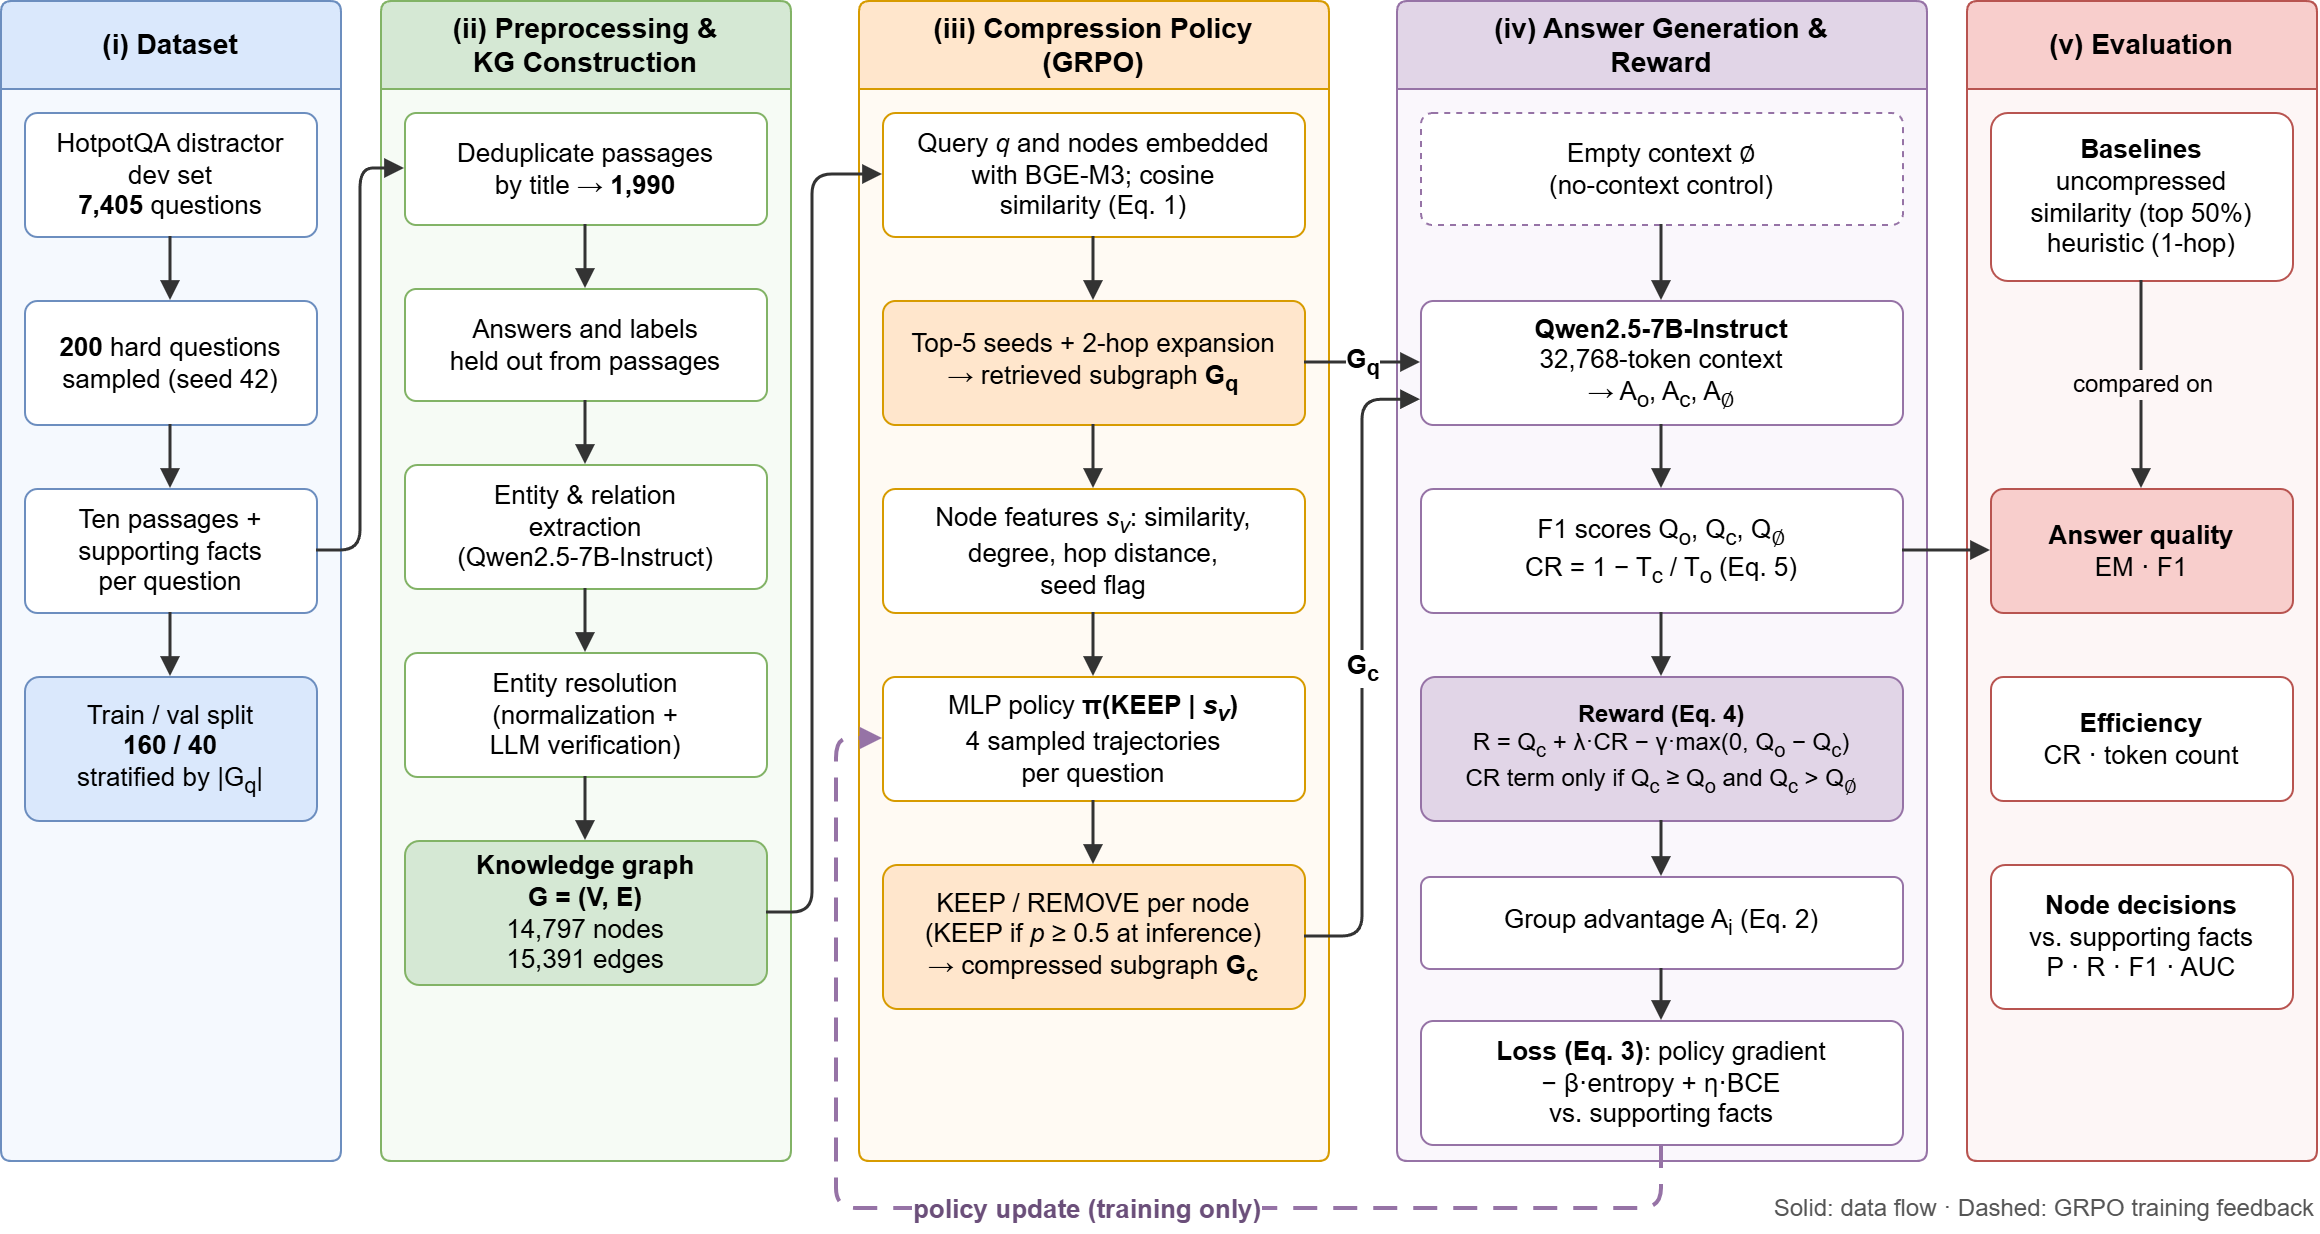
\includegraphics[width=0.95\linewidth]{workflow_diagram.jpg}
    \caption{Overview of the proposed adaptive graph compression workflow. Retrieved subgraph $G_q$ is processed with GRPO-based compression to $G_c$ (answer $A_c$) and without RL compression (answer $A_o$); token ratio and reward/penalty are computed by comparing $A_c$ against $A_o$, which in turn updates the compression policy.}
    \label{fig:workflow}
\end{figure*}

\subsection{Dataset and Knowledge Graph Construction}

The framework is evaluated on HotpotQA \cite{yang2018hotpotqa}, a multi-hop question-answering benchmark in which correctly answering a query requires synthesizing evidence distributed across multiple supporting documents rather than a single passage. This multi-hop dependency structure makes HotpotQA well-suited to graph-based retrieval, since the entities and relations connecting disjoint evidence fragments can be explicitly represented as graph structure rather than left implicit in flat text chunks, and it makes the corpus similarly well-suited to studying compression, since not all retrieved nodes and edges contribute equally to the final reasoning chain.

Supporting documents are converted into a knowledge graph using Qwen2.5-7B-Instruct \cite{qwen2024technical}, which performs entity identification and relation extraction over the source text. Coreferent mentions are then merged in two stages. First, mentions already linked by an explicit alias relation stated in the source text (e.g., ``was known as'') are merged directly at no additional verification cost, since the alias is already an extracted fact. Second, remaining same-name mentions and fuzzy-matched candidates (sharing an entity type and a distinctive name token) are each verified by a dedicated LLM call that assigns a relationship category -- \textit{identical}, \textit{part-of}, \textit{different individual}, \textit{related work}, \textit{coincidental same name}, or \textit{unclear} -- rather than a binary same/different judgment, which we found more robust to the extraction model's inconsistent free-text reasoning on this task. This second stage is necessary because naive name-based merging alone both misses genuine aliases with different wording and incorrectly conflates distinct entities that merely share a name or title (e.g., unrelated works with an identical title), while categorical verification additionally distinguishes relationships a flat merge would conflate (e.g., a legislative chamber from its parent legislature). A manual audit of one full construction run (1,975 verified pairs) found a residual error rate of approximately 0.76\% after targeted prompt refinements; we report this as an empirically observed error ceiling for this extraction model on this task rather than a fully eliminated source of error. The resulting knowledge graph is represented as $G = (V, E)$, where $V$ denotes the set of entity nodes and $E$ denotes the set of semantic relations connecting them. This graph serves as the persistent knowledge structure over which retrieval and compression are subsequently performed.

\subsection{Query Representation and GraphRAG Retrieval}

To enable semantic matching between queries and graph elements, BGE-M3 \cite{chen2024bgem3} is used to embed both the query and each graph node. Given a query $q$, its embedding is computed as $E_q = \mathrm{BGE\text{-}M3}(q)$, and for each node $v_i \in V$, $E_i = \mathrm{BGE\text{-}M3}(v_i)$. Semantic relevance between the query and a given node is quantified using cosine similarity,
\begin{equation}
    \mathrm{sim}(q, v_i) = \mathrm{cosine}(E_q, E_i),
    \label{eq:sim}
\end{equation}
which provides the basis for GraphRAG's retrieval decisions.

Given the full graph $G$ and query $q$, we retrieve a candidate subgraph $G_q = (V_q, E_q)$ using a top-$k$ semantic-seed and $k$-hop expansion strategy: the $k$ nodes of highest similarity to $q$ (Eq.~\ref{eq:sim}) are selected as seeds, and $G_q$ is grown by expanding outward along undirected graph edges up to a fixed hop limit. This adopts the general GraphRAG principle of retrieving a query-relevant subgraph prior to generation \cite{edge2024local}, but differs from the hierarchical community-summary retrieval of \citet{edge2024local} in that no community detection or summarization is performed; expansion beyond pure top-$k$ similarity is necessary because a fact required for a multi-hop answer is often not itself semantically close to the query and is reachable only by traversing the graph from a jointly-relevant entity. It is important to distinguish the roles of the two subsequent stages: retrieval determines which graph information may be relevant to the query, while compression determines which of that retrieved information should actually be retained for generation. This separation is central to the framework's contribution, as it decouples the coverage-oriented retrieval objective from the efficiency-oriented compression objective.

\subsection{Answer Generation from the Retrieved Graph}

Following retrieval of the candidate subgraph $G_q = (V_q, E_q)$ by GraphRAG, the retrieved graph is used as input to Qwen2.5-7B-Instruct \cite{qwen2024technical} without any reinforcement learning or graph compression. The retrieved entities, relations, and their textual evidence are collected into the query-specific context that is sent to the language model alongside query $q$. The model generates the answer $A_o$ in the context of the retrieved information. This step sets the baseline performance of the GraphRAG method in the uncompressed variant and provides the original context and answer to compare against in the compression stage.

The answer is evaluated against the reference answer for the query, whereas the retrieved context is saved for further processing. The result of this step is the original retrieved context, its token count $T_o$, and the generated answer $A_o$. At this step, no pruning or learned policy is used; the retrieved subgraph $G_q$ is subsequently fed into the query-adaptive compression module, which learns to retrieve a smaller subgraph while preserving the answer quality of the GraphRAG baseline.

\subsection{GRPO-Based Query-Adaptive Graph Compression}

The retrieved subgraph $G_q$, while relevant, typically contains redundant or peripheral nodes that do not contribute to the multi-hop reasoning chain required to answer $q$. The compression stage therefore learns a policy that produces a reduced subgraph $G_c \subseteq G_q$, preserving information necessary for downstream QA while discarding non-essential structure. The policy operates at node granularity, assigning each node in $G_q$ an action from $\mathcal{A} = \{\mathrm{KEEP}, \mathrm{REMOVE}\}$. The policy's decision state is constructed from query and graph information, including the query embedding, node representations, query-node semantic relevance scores, and graph-context features -- specifically each node's degree within $G_q$ (normalized by the maximum degree in $G_q$), its hop-distance from the nearest retrieval seed (normalized by the maximum such distance in $G_q$), and a binary indicator of whether the node is itself a retrieval seed.

The policy is trained using GRPO \cite{shao2024deepseekmath}, in which multiple candidate compression trajectories are sampled for the same query-graph context, each trajectory's downstream reward is computed, and trajectories are compared relative to one another within the group rather than against an absolute value baseline. This relative comparison yields a conceptual advantage estimate for candidate $i$,
\begin{equation}
    A_i = \frac{R_i - \mu_R}{\sigma_R + \epsilon},
    \label{eq:advantage}
\end{equation}
where $R_i$ is the reward of candidate $i$, $\mu_R$ and $\sigma_R$ are the group's mean and standard deviation of rewards, and $\epsilon$ is a small constant added for numerical stability. This group-relative formulation allows the policy to be optimized without a separately trained value/critic network.

\subsection{Compressed Answer Generation and Reward}

Each compressed graph $G_c$ is passed to Qwen2.5-7B-Instruct \cite{qwen2024technical} to generate answer $A_c$, which is compared against baseline $A_o$ from Section~III-C. The compression ratio is defined as
\begin{equation}
    CR = 1 - \frac{T_c}{T_o},
    \label{eq:cr}
\end{equation}
and QA quality is defined as
\begin{equation}
    Q_c = \mathrm{sim}(A_c, A_{gt}),
    \label{eq:qc}
\end{equation}
where $A_{gt}$ is the ground-truth answer and $\mathrm{sim}(\cdot)$ is a similarity/correctness score; we use token-level F1 against the ground-truth answer, consistent with the QA evaluation metric of Section~III-F, though the formulation admits alternative scores such as ROUGE or LLM-judged accuracy. The degradation penalty is defined as
\begin{equation}
    P = \max(0,\, Q_o - Q_c),
    \label{eq:penalty}
\end{equation}
where $Q_o = \mathrm{sim}(A_o, A_{gt})$, so $P > 0$ only when the compressed answer underperforms the baseline. The joint reward is then
\begin{equation}
    R = Q_c + \lambda \cdot CR \cdot \mathbb{1}[Q_c \geq Q_o] - \gamma P,
    \label{eq:reward}
\end{equation}
where $\mathbb{1}[\cdot]$ is the indicator function: the compression bonus is credited only when compression has not reduced answer quality below the uncompressed baseline. This gating is necessary rather than cosmetic -- an unconditional compression bonus ($R = Q_c + \lambda CR - \gamma P$) makes emptying the graph entirely a dominant strategy whenever the downstream generator can still answer correctly from parametric knowledge alone despite an empty context, or whenever the uncompressed baseline was already incorrect ($Q_o$ low, so $P \approx 0$ regardless of $Q_c$); both conditions occur often enough on a multi-hop QA benchmark with a capable generator to collapse an ungated policy to removing all context on every query, which we verified empirically. Gating the bonus on $Q_c \geq Q_o$ removes this degenerate incentive while preserving the intended compression-quality trade-off. The GRPO advantage, given in \eqref{eq:advantage} and repeated here for completeness,
\begin{equation}
    A_i = \frac{R_i - \mu_R}{\sigma_R + \epsilon},
    \label{eq:advantage2}
\end{equation}
is computed after the reward/penalty step to rank candidates and update the compression policy.

\subsection{Performance and Evaluation}

The proposed framework is evaluated along two axes: QA effectiveness and compression efficiency. QA effectiveness is measured using Exact Match (EM) and F1 score. Compression efficiency is measured via the original and compressed context token counts, $T_o$ and $T_c$, and the token reduction percentage:
\begin{equation}
    \text{Token Reduction (\%)} = \frac{T_o - T_c}{T_o} \times 100.
    \label{eq:tokenreduction}
\end{equation}
Successful compression is defined as a meaningful reduction in context size without unacceptable degradation in QA performance.

The proposed GRPO-compressed pipeline is directly and mandatorily compared against the original uncompressed GraphRAG pipeline, which serves as the baseline, consistent with Section~III-E. The original GraphRAG constitutes the baseline method, producing $A_o$, while the GRPO-compressed GraphRAG constitutes the proposed method, producing $A_c$. The two are evaluated using EM and F1 to determine whether compression preserves baseline QA performance:
\begin{equation}
    \Delta EM = EM(A_o) - EM(A_c), \quad \Delta F1 = F1(A_o) - F1(A_c).
    \label{eq:delta}
\end{equation}
Compression efficiency is assessed via $T_o$, $T_c$, and token reduction (\ref{eq:tokenreduction}). The QA-performance difference between $A_o$ and $A_c$ is used to determine the reward or penalty assigned to the RL agent, as defined in Section~III-D and III-E.

Additional comparisons with two non-adaptive pruning strategies are included to assess whether the query-adaptive, reward-driven compression strategy achieves a superior trade-off between answer quality and context reduction relative to non-adaptive alternatives: (i) \textit{similarity-based pruning}, which retains a fixed top fraction of $G_q$'s nodes ranked by query-node cosine similarity (Eq.~\ref{eq:sim}), independent of graph structure; and (ii) \textit{fixed/heuristic pruning}, which retains only nodes within a fixed hop distance of a retrieval seed within $G_q$, independent of query semantics. Neither baseline adapts its retention decision to the specific query or to downstream answer quality, in contrast to the learned policy of Section~III-D.
